\newpage

\chapter{About the school}

Three types of events are hosted by the school:

\section{The Summer School sessions}

The summer school sessions are aimed primarily towards advanced students and young postdoctoral researchers, willing to deepen their knowledge or to start in a new field.

The sessions last from 4 to 5 weeks and the courses are long (up to 12 hours of lectures for a given subject). This allows a thorough pedagogical approach, up to the frontiers of modern research, and to cover all aspects of a given subject. This long duration also favors exchanges, discussions and working groups between participants.

The summer school programs are selected by the Board about two years in advance. If you have suggestions, or if you are interested in organizing a session, contact the Director of the School.

\section{The Workshops}

The rest of the year is dedicated to workshops, lasting one, two or sometimes three weeks, which bring together theoreticians and experimentalists. Participants exchange knowledge and are confronted by different view points that may lead to the definition of new research programmes. Meetings of the Center of Physics are usually organised in order to leave enough time for discussion in groups that meet in small, separate work rooms.

Any project of workshop at the Center must be first discussed with the Director of the School.


\section{The Predoctoral School}


The Predoctoral School brings together young beginners in scientific
research.The aim of the Predoctoral School is to help them acquire a
broader base in physics and place their thesis work in proper
context. It can also prepare them for a richer scientific career by
avoiding too much specialisation too early.


\chapter{History}

Les Houches School of Physics has been welcoming physicists from around the world since 1951. The School has seen the biggest names in modern physics training young researchers at the start of their careers, some of whom have since won Nobel prizes for physics. The school perpetuates a tradition of excellence, while continuing to adapt to the evolutions of science.

\section{The origins of the school}

Les Houches School of Physics was founded in 1951 by a young French physicist, Cécile DeWitt-Morette. She wanted to help to rebuild her country, which, like so many others in the wake of the war, was lagging seriously behind in the teaching and practice of modern physics.

The dynamic and visionary Cécile DeWitt-Morette succeeded in building a school, with the few resources available, to which leading world specialists would come to share their knowledge with groups of around thirty students from different countries (mostly France and other European countries, but not only). The setting is idyllic, lying above the Chamonix valley, in full view of the Mont-Blanc mountains. However, back then, living conditions were very rudimentary: the sessions lasted eight weeks (the two months of the university summer holidays), staying in mountain chalets will no facilities, a few kilometres from Les Houches village.

\section{Immediate recognition}

History relates that the first class, on quantic mechanics, was held in 1951 by Léon van Hove. The school quickly attracted interest from the biggest names in physics, including Enrico Fermi, Wolfgang Pauli, Murray Gell-Mann and John Bardeen, to name but a few. Cécile DeWitt-Morette also promoted unknown youngsters: in 1951, Walter Kohn (1998 Nobel prize for chemistry), aged 28, gave a class on solid state physics. Philippe Nozières was asked to organise a session on the N-body problem in 1958, when he was just 26 years old. The school’s students have included Pierre-Gilles de Gennes, Georges Charpak, and Claude Cohen-Tannoudji, future winners of the Nobel prize for physics, and later on, mathematician Alain Connes (Fields medal 1982). All have had the opportunity to testify their immense gratitude to the school.

\newpage

\begin{itemize}
\item  Nobel prizes who came to les Houches:

\begin{multicols}{2}
{\footnotesize
P.W. Anderson,
came to les Houches in 1967. Nobel prize in 1977.

J. Bardeen,
came to les Houches in 1956. Nobel prizes in 1956 and 1972.

N. Bloembergen ,
came to les Houches in 1964. Nobel prize in 1981.

A. Bohr,
came to les Houches in 1955. Nobel prize in 1975.

A. Chamberlain,
came to les Houches in 1957. Nobel prize in 1959.

S. Chu,
came to les Houches in 1999. Nobel prize in 1997.

C. Cohen-Tannoudji,
came to les Houches in 1964. Nobel prize in 1997.

A. Connes,
came to les Houches in 1970. Fields Medalist in 1982.

L.N. Cooper,
came to les Houches. Nobel prize in 1972.

E.A. Cornell,
came to les Houches in 1999. Nobel prize in 2001.

F. Englert,
came to les Houches in 1979. Nobel prize in 2013.

E. Fermi,
came to les Houches in 1954. Nobel prize in 1938.

R. Feynman,
came to les Houches in 1976. Nobel prize in 1965.

R. Glauber,
came to les Houches in 1954 and 1964. Nobel prize in 2005.

M. Gell-Mann,
came to les Houches in 1952. Nobel prize in 1969.

P.G. de Gennes,
came to les Houches in 1953 and 1967. Nobel prize in 1991.

D.J. Gross,
came to les Houches in 1975. Nobel prize in 2004.

D.M. Haldane,
came to les Houches in 2008. Nobel prize in 2016.

S. Haroche,
came to les Houches in 1990. Nobel prize in 2012.

G. Hooft,
came to les Houches in 1975. Nobel prize in 1999.

J.H. Jensen,
came to les Houches in 1953. Nobel prize in 1963.

A. Kastler,
came to les Houches in 1951. Nobel prize in 1966.

W. Ketterle,
came to les Houches in 1999 and 2010. Nobel prize in 2001.

W. Kohn,
came to les Houches in 1951 and 1967. Nobel prize in 2003.

W. Lamb,
came to les Houches in 1964. Nobel prize in 1955.

T.D. Lee,
came to les Houches in 1975. Nobel prize in 1957.

A. Leggett,
came to les Houches in 1986. Nobel prize in 2003.

A.B. McDonald,
came to les Houches in 1994. Nobel prize in 2015.

B. Mottelson,
came to les Houches in 1958. Nobel prize in 1975.

L. Néel,
came to les Houches in 1956 and 1961. Nobel prize in 1970.

W. Pauli,
came to les Houches in 1951, 1952 and 1955. Nobel prize in 1945.

A. Penzias,
came to les Houches in 1974. Nobel prize in 1978.

W.D. Phillips,
came to les Houches in 1999 and 2010. Nobel prize in 1997.

N. Ramsey,
came to les Houches in 1955. Nobel prize in 1989.

A. Salam,
came to les Houches in 1957. Nobel prize in 1979.

E. Segré,
came to les Houches in 1951. Nobel prize in 1959.

B. Schmidt,
came to les Houches in 1990. Nobel prize in 2011.

J.R. Schrieffer,
came to les Houches in 1958. Nobel prize in 1972.

J. Schwinger,
came to les Houches in 1955. Nobel prize in 1965.

W. Shockley,
came to les Houches in 1953. Nobel prize in 1956.

J. Steinberger,
came to les Houches in 1960. Nobel prize in 1988.

R. Thom,
came to les Houches. Fields Medalist in 1958.

K. S. Thorne,
came to Les Houches in 1963, 1966, 1972, 1982. Nobel prize in 2017.

D.J. Thouless,
came to les Houches in 1978. Nobel prize in 2016.

C. Townes,
came to les Houches in 1955. Nobel prize in 1964.

JG Veltman,
came to les Houches in 1976. Nobel prize in 1999.

EP Wigner,
came to les Houches in 1955. Nobel prize in 1963.

KG Wilson,
came to les Houches in 1975. Nobel prize in 1982.

E. Witten,
came to les Houches. Fields Medalist in 1990.

C.N. Yang,
came to les Houches in 1957. Nobel prize in 1958.
}
\end{multicols}

\item  Famous professors and students who came to les Houches
\begin{multicols}{2}

ALAIN CONNES,\\
Fields Medalist 1982
 
CLAUDE COHEN TANNOUDJI,\\
Nobel Prize 1997
 
ENRICO FERMI,\\
Nobel Prize 1938
 
JOHN BARDEEN,\\
Nobel Prize 1956 and 1972
 
LEON VAN HOVE,\\
CERN director 1976-1980
 
PIERRE GILLES DE GENNES,\\
Nobel prize 1991
 
RICHARD FEYNMAN,\\
Nobel Prize 1965
 
WOLFGANG PAULI,\\
Nobel Prize 1945
\end{multicols}


\end{itemize}

During the 1950s and 60s, Les Houches School of Physics had a considerable impact on the development of top level physics in France and beyond. Its operational concept has been copied throughout the world. NATO, through Norman Ramsey, very quickly offered its support to the school, and launched its Advanced Study Institutes in 1958, based on the model of Les Houches.

\section{The school today}

The school has changed over the years, although some of its traditions have been preserved and it continues to attract world leaders in the field. The main events of the year remain the two summer schools (in-depth, month-long courses in July and August on innovative themes). These form a kind of post-doctoral school, which has remained something of a trademark for Les Houches. Various courses and shorter, more specialised conferences are organised throughout the year in the “Physics Centre”. Some are intended for all researchers (from beginners to experts) while others are primarily designed for post-graduate students (doctoral courses). Aside from the educational aspects, these meetings also enable the development of scientific collaborations. Effective professional and social networks are frequent by-products of Les Houches schools.

The school has kept up with the evolutions of science, opening up to peripheral fields, such as mathematics, earth sciences, chemistry and biology. The interactions between these disciplines are actually very often at the core of the issues investigated nowadays in Les Houches.

\section{Major milestones}

\begin{itemize}

\item 1977: creation of the "Physics Centre"

\item More specialised, shorter conferences are now organised all year round, with the specific ambition of promoting more original themes, bringing together physicists from different cultures and scientists from different disciplines.
1988: creation of the "Pre-doctoral School"

More general courses for young researchers working on their theses, or
even before starting. Today, the term "doctoral course" is more
commonly used.

\end{itemize}

\newpage

\chapter{Access}

\section{By plane}

Geneva Airport is 1 hour drive from les Houches. 
Once you have landed, you can reach the school using a shuttle service, the regular bus service or by train.

\subsection{Shuttle service}

The simplest way is to use a shuttle service (approximately 40 euros up to the school, book at least three days in advance). If you already have your return date, we would recommend to book a return trip.
> Consult the list of companies

Beware: we do not recommend the Alpybus company (they do not reach the school).

Price discounts are available with Mountain Drop-Offs. To find Mountain Drop-Offs' meeting point easily in the Geneva Airport please consult the video How to find Mountain Drop-Offs at Geneva Airport.

\subsection{Regular bus service}

There is also a regular bus service between Geneva and Les Houches (only once or twice a day). One should then take a taxi for the last 5 kms from the Les Houches village to the school (the total cost is similar to that of the limousine).

\subsection{Train}

One can also travel from Geneva to Les Houches by train (+ taxi from the train station to the School), but it is quite complicated (3 connections) and long (go through Annemasse on the French side or through Martigny on the Swiss side).

\section{By train}

Arrival at the Les Houches station, with one change at Saint-Gervais (from France), or at Martigny (from Switzerland). 
There are about 10 trains per day between St Gervais and Les Houches (schedules, 20mn trip). 
Then we strongly advise you to take a taxi to go up to the school (5km).

Taxi phone numbers :
\begin{itemize}
\item (+33/0)6-07-26-36-62,
\item (+33/0)6.22.75.19.37,
\item (+33/ 0)6.12.35.30.72.
\end{itemize}

\section{By road}

Les Houches are easily accessible from France (A41 highway), from Switzerland (Martigny and Col des Montets) and from Italy through the Mont Blanc Tunnel.
From Geneva and Le Fayet

8km before Chamonix, 300 m after passing under the tunnel, bear right
by the first road out for "Les Houches Bellevue". When arriving at the
cable car station "Bellevue", turn right and continue upwards (roughly
2 km starting from the teleferic). 500m after the cable car station
"Prarion", turn left and follow small arrows at crossroads. Continue
up to the end of Route de la Côte des Chavants. Here you are!

\subsection{From Chamonix}

Bear right for "Les Houches-Chef-Lieu", turn right in Les Houches, go ahead at the cable car station "Bellevue". Then proceed as above.

Cars may be rented from Geneva and from Chamonix, it is useful to make a reservation.
What to do in Les Houches and in the valley?

See for example: {\ttfamily http://www.leshouches.com} and
{\ttfamily http://www.chamonix.com}

\vspace{1cm}

ADDRESS OF THE SCHOOL:\\
\\
Les Houches School of Physics\\
140 Chemin de la Côte\\
F-74310 Les Houches\\

\chapter{Open street maps}


\begin{figure}[!ht]
  \includegraphics[width=\textwidth]{intros/map_2.pdf}  
  \caption{Village de Chamonix}
  \label{FIG1}
\end{figure}


\begin{figure}[!ht]
  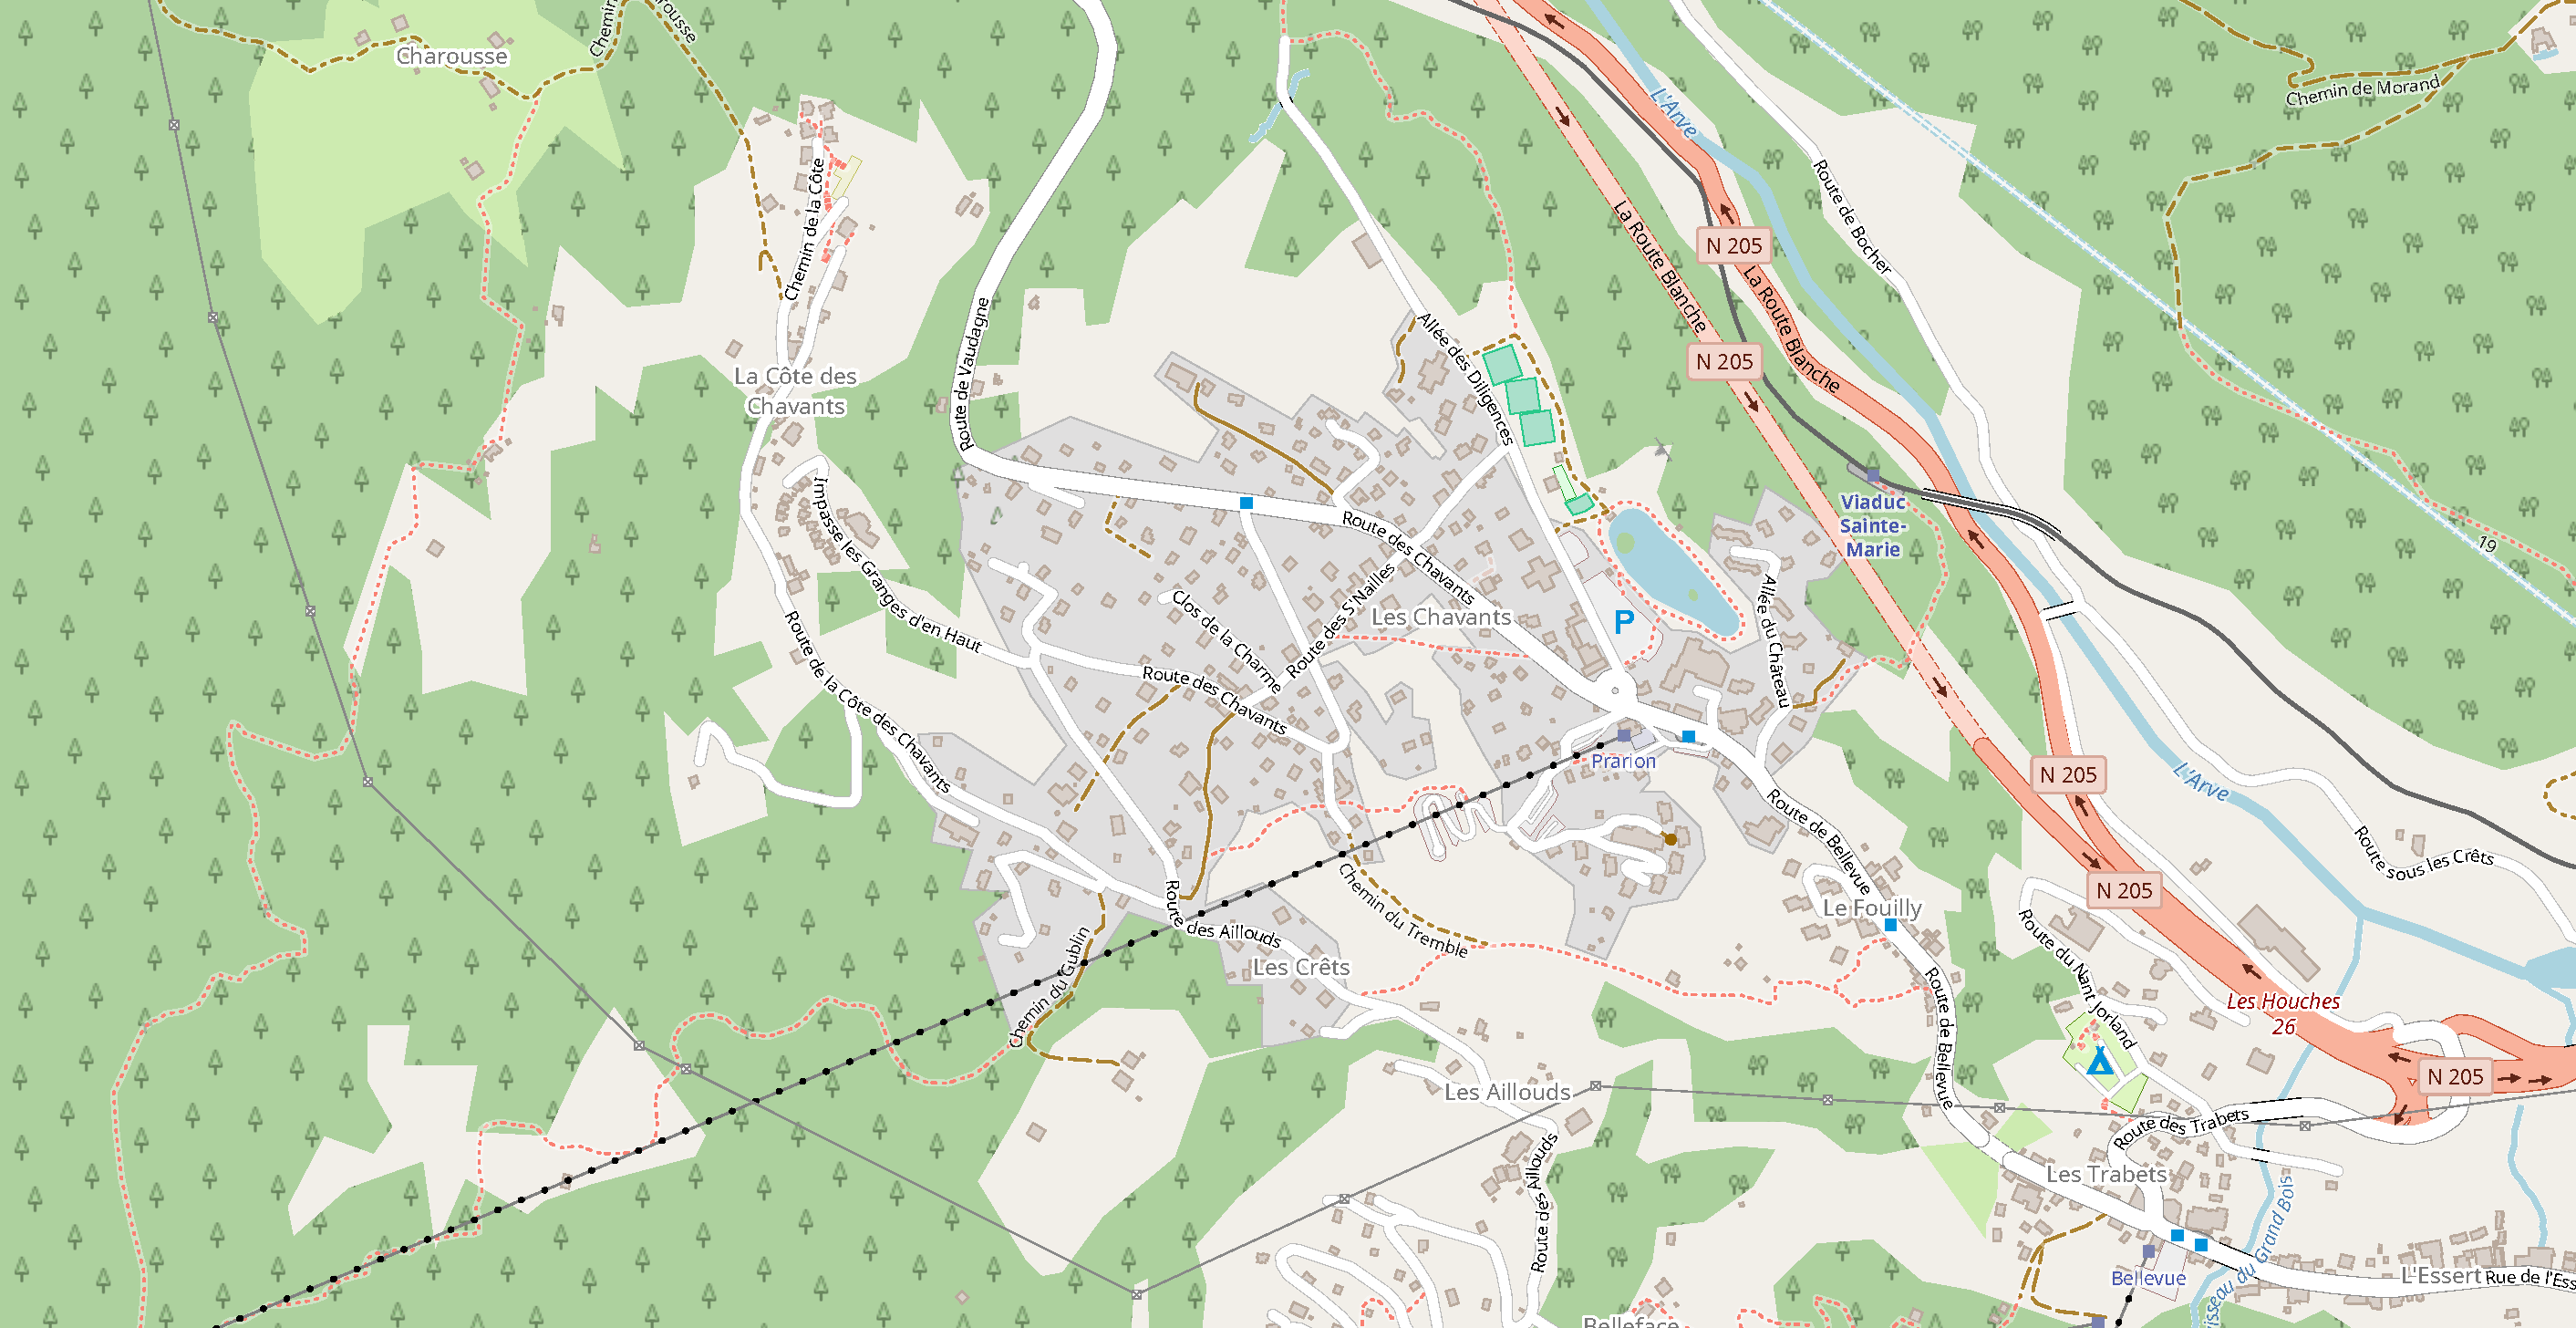
\includegraphics[width=\textwidth]{intros/map_1.pdf}  
  \caption{Hameaux des Houches}
  \label{FIG1}
\end{figure}

\chapter{Map of the \'Ecole de Physique}

\includegraphics[width=\textwidth]{intros/practical_info_Houches.pdf}
% \begin{figure}
  
%   \caption{\'Ecole de Physique des Houches}
%   \label{FIG1}
% \end{figure}


\chapter{Ski slopes: Prarion $-$ Saint-Gervais}

\includegraphics[width=\textwidth]{intros/Plan_Hiver_HCH.pdf}
% \begin{figure}
 
%   \caption{\'Ecole de Physique des Houches}
%   \label{FIG1}
% \end{figure}

\newpage